%============================================================
% BAB 3 — hasil konversi awal dari DOCX lama
%============================================================
\chapter{DESKRIPSI SISTEM}

Bab ini menjelaskan rancangan solusi yang diusulkan untuk mendeteksi potensi fraud atau upcoding pada data klaim kesehatan JKN/BPJS. Penyajian bab disusun mengikuti alur pipeline penelitian, yaitu dimulai dari pembentukan dataset claim-centric, dilanjutkan dengan pembentukan pseudo-label, benchmarking model supervised, penentuan threshold keputusan, dan diakhiri dengan evaluasi serta interpretabilitas hasil. Dengan susunan tersebut, pembaca diharapkan dapat memahami hubungan antara sumber data, tahapan analisis, dan keluaran sistem yang dihasilkan secara lebih runtut.

Perancangan sistem pada penelitian ini berlandaskan pada pendekatan berbasis klaim atau~\emph{claim-centric}, yaitu menjadikan satu klaim sebagai unit analisis utama. Dengan pendekatan tersebut, sistem tidak hanya memeriksa nilai biaya klaim secara terpisah, tetapi juga mengaitkannya dengan informasi kepesertaan, diagnosis sekunder, histori layanan, dan karakteristik klinis yang relevan. Rancangan ini dipilih agar proses deteksi tidak berhenti pada identifikasi anomali, tetapi juga mampu memberikan dasar analitis yang lebih kuat untuk menjelaskan mengapa suatu klaim diprediksi berisiko.

\section{DESKRIPSI SOLUSI}\label{deskripsi-solusi}

Solusi yang diajukan pada penelitian ini adalah sistem deteksi potensi \emph{fraud} atau \emph{upcoding} pada klaim kesehatan JKN/BPJS berbasis~\emph{machine learning}~dengan pendekatan~\emph{claim-centric}. Sistem ini dirancang untuk membantu proses identifikasi klaim yang memiliki tingkat risiko tinggi berdasarkan pola biaya, kondisi klinis, atribut peserta, dan riwayat layanan kesehatan yang tercatat pada data klaim. Fokus utama penelitian bukan untuk menetapkan bahwa suatu klaim terbukti \emph{fraud} secara hukum, melainkan untuk membangun mekanisme analitis yang mampu menandai klaim-klaim yang patut diprioritaskan untuk pemeriksaan lebih lanjut.

Pendekatan~\emph{claim-centric}~digunakan dengan menjadikan tabel~FKRTL~sebagai pusat analisis. Setiap baris data merepresentasikan satu klaim, kemudian diperkaya dengan informasi dari tabel lain, seperti data kepesertaan, diagnosis sekunder, serta histori layanan sebelumnya dari layanan FKTP dan nonkapitasi. Dengan rancangan ini, sistem dapat memandang klaim sebagai satu entitas yang utuh, bukan hanya sebagai catatan biaya, sehingga deteksi risiko dapat mempertimbangkan konteks administratif, klinis, dan historis secara bersamaan.

Untuk menangani keterbatasan utama berupa tidak tersedianya label \emph{fraud} transaksi riil pada level klaim, penelitian ini menggunakan pendekatan~\emph{hybrid fraud detection modeling}. Pada tahap awal, sistem menerapkan~\emph{Isolation Forest}~untuk melakukan~\emph{pseudo-labeling}~terhadap klaim yang memiliki pola anomali. Pseudo-label ini kemudian digunakan sebagai target pada tahap~\emph{supervised learning}~agar model dapat mempelajari pola yang membedakan klaim berisiko dan klaim normal. Pendekatan ini dipilih karena memungkinkan penelitian tetap membangun model prediktif meskipun tidak tersedia label \emph{fraud} final yang siap pakai.

Setelah \emph{pseudo-label} terbentuk, sistem melakukan~\emph{benchmarking}~terhadap beberapa model~\emph{supervised learning}~untuk memperoleh model dengan performa terbaik. Strategi ini digunakan agar pemilihan model tidak didasarkan pada asumsi awal terhadap satu algoritma tertentu, tetapi pada hasil evaluasi \emph{empiris} dari beberapa kandidat model. Dengan demikian, model final yang dipilih benar-benar merepresentasikan konfigurasi yang paling sesuai terhadap karakteristik data klaim yang digunakan dalam penelitian ini.

Selain menekankan performa prediksi, solusi yang diusulkan juga menempatkan interpretabilitas sebagai komponen penting. Interpretabilitas diperlukan agar hasil prediksi model tidak berhenti pada pemberian skor risiko, tetapi juga dapat dijelaskan melalui fitur-fitur yang berkontribusi terhadap keputusan model, baik pada tingkat global maupun lokal. Hal ini penting karena domain klaim kesehatan menuntut hasil analisis yang tidak hanya akurat, tetapi juga dapat dipahami dan dipertanggungjawabkan. Oleh sebab itu, sistem ini dirancang untuk menghasilkan deteksi potensi fraud yang terstruktur, terukur, dan dapat dijelaskan secara analitis.

\phantomsection\label{_Toc228109620}{}Tabel 3. 1 Komponen Utama Solusi yang Diusulkan

\begin{longtable}[]{@{}
  >{\raggedright\arraybackslash}p{(\columnwidth - 4\tabcolsep) * \real{0.2524}}
  >{\raggedright\arraybackslash}p{(\columnwidth - 4\tabcolsep) * \real{0.3411}}
  >{\raggedright\arraybackslash}p{(\columnwidth - 4\tabcolsep) * \real{0.4065}}@{}}
\toprule\noalign{}
\begin{minipage}[b]{\linewidth}\raggedright
\textbf{Komponen}
\end{minipage} & \begin{minipage}[b]{\linewidth}\raggedright
\textbf{Fungsi}
\end{minipage} & \begin{minipage}[b]{\linewidth}\raggedright
\textbf{Kontribusi dalam Sistem}
\end{minipage} \\
\midrule\noalign{}
\endhead
\bottomrule\noalign{}
\endlastfoot
\emph{Claim-centric integration} & Menjadikan klaim sebagai unit analisis utama & Menyatukan informasi klaim, peserta, diagnosis, dan histori layanan \\
\emph{Pseudo-labeling} & Membentuk label awal berbasis anomali & Mengatasi ketiadaan label \emph{fraud} transaksi riil \\
\emph{Supervised benchmarking} & Membandingkan beberapa model klasifikasi & Memilih model terbaik berdasarkan hasil evaluasi \\
\emph{Threshold tuning} & Menentukan ambang klasifikasi optimal & Menyesuaikan keputusan akhir model \\
\emph{Interpretability} & Menjelaskan hasil prediksi model & Mendukung pemahaman faktor risiko klaim \\
\end{longtable}

Tabel 3.1 merangkum komponen utama solusi yang diusulkan dalam penelitian ini. Setiap komponen memiliki peran yang saling terhubung, mulai dari pembentukan dataset berbasis klaim, pembentukan \emph{pseudo-label}, pemilihan model terbaik, hingga penjelasan terhadap hasil prediksi.

\section{\texorpdfstring{PERANCANGAN SISTEM}{PERANCANGAN SISTEM}}\label{perancangan-sistem}

Bagian ini menjelaskan desain sistem secara teknis dan runtut, mulai dari tahap persiapan data berbasis klaim, proses pemodelan deteksi fraud secara hybrid, hingga tahap evaluasi dan interpretabilitas hasil. Perancangan sistem disusun dalam bentuk alur bertahap agar hubungan antara data masukan, proses analisis, dan keluaran sistem dapat dipahami secara menyeluruh. Dengan rancangan ini, sistem tidak hanya berfungsi untuk menghasilkan prediksi risiko, tetapi juga menyediakan dasar analitis yang dapat digunakan untuk menjelaskan alasan di balik prediksi tersebut.

Secara umum, desain sistem pada penelitian ini terdiri atas tiga komponen utama, yaitu~\emph{Claim-Centric Data Preparation},~\emph{Hybrid Fraud Detection Modeling}, dan~\emph{Evaluation and Interpretability}. Komponen pertama berfokus pada penyiapan data mentah menjadi dataset analisis berbasis klaim. Komponen kedua berfokus pada pembentukan pseudo-label, pembandingan model, dan pemilihan model terbaik. Komponen ketiga berfokus pada evaluasi model final dan interpretasi hasil prediksi. Hubungan antar ketiga komponen tersebut ditunjukkan pada Gambar 3.1.

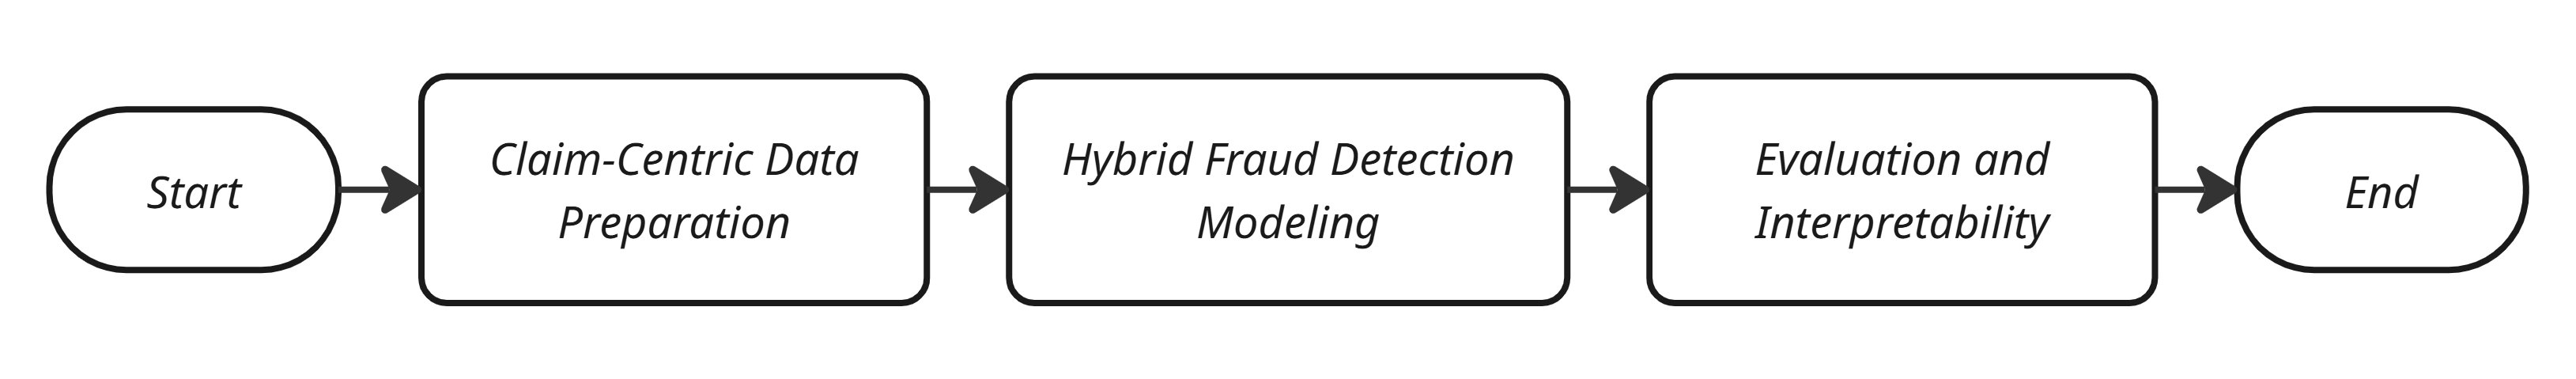
\includegraphics[width=5.51181in,height=0.81042in]{media/media/image6.png}

\phantomsection\label{_Toc228109334}{}Gambar 3. 1 Desain Sistem Deteksi Potensi Fraud Klaim

Berdasarkan Gambar 3.1, alur sistem dimulai dari tahap persiapan data berbasis klaim untuk membentuk dataset analitis yang terstruktur. Dataset tersebut selanjutnya digunakan pada tahap~\emph{hybrid fraud detection modeling}~untuk membangun model deteksi risiko berbasis pseudo-label dan~\emph{supervised learning}. Setelah model final diperoleh, proses dilanjutkan ke tahap evaluasi dan interpretabilitas guna menilai performa model serta menjelaskan faktor-faktor yang berkontribusi terhadap prediksi klaim berisiko tinggi. Untuk memberikan pembahasan yang lebih rinci, masing-masing komponen utama tersebut dijelaskan pada subbagian berikutnya.

\subsection{\texorpdfstring{\emph{Claim-Centric Data Preparation}}{Claim-Centric Data Preparation}}\label{claim-centric-data-preparation}

Tahap~\emph{Claim-Centric Data Preparation}~merupakan bagian awal dari sistem yang bertujuan mengubah data mentah BPJS menjadi dataset analisis berbasis klaim. Pada tahap ini, setiap klaim diposisikan sebagai unit analisis utama, sehingga seluruh proses integrasi, pembersihan, dan pembentukan fitur diarahkan untuk menghasilkan satu representasi data yang utuh pada level klaim. Pendekatan ini dipilih agar deteksi potensi fraud tidak hanya mengandalkan satu atribut biaya, tetapi juga mempertimbangkan konteks peserta, diagnosis, histori layanan, dan karakteristik klinis yang menyertai klaim tersebut.

Sumber data yang digunakan pada penelitian ini terdiri atas beberapa tabel utama, yaitu~FKRTL,~kepesertaan,~diagnosissekunder,~FKTP kapitasi, dan~nonkapitasi. Masing-masing tabel memiliki fungsi yang berbeda dalam \emph{pipeline} analisis, mulai dari penyediaan informasi inti klaim, data profil peserta, rincian diagnosis tambahan, hingga histori pemanfaatan layanan sebelum terjadinya klaim. Ringkasan fungsi setiap tabel dan perannya dalam pipeline ditunjukkan pada Tabel 3.2.

\phantomsection\label{_Toc228109621}{}Tabel 3. 2 Tabel Sumber Data yang Digunakan

\begin{longtable}[]{@{}
  >{\raggedright\arraybackslash}p{(\columnwidth - 4\tabcolsep) * \real{0.2510}}
  >{\raggedright\arraybackslash}p{(\columnwidth - 4\tabcolsep) * \real{0.3776}}
  >{\raggedright\arraybackslash}p{(\columnwidth - 4\tabcolsep) * \real{0.3714}}@{}}
\toprule\noalign{}
\begin{minipage}[b]{\linewidth}\raggedright
\textbf{Nama Tabel}
\end{minipage} & \begin{minipage}[b]{\linewidth}\raggedright
\textbf{Fungsi}
\end{minipage} & \begin{minipage}[b]{\linewidth}\raggedright
\textbf{Peran dalam \emph{Pipeline}}
\end{minipage} \\
\midrule\noalign{}
\endhead
\bottomrule\noalign{}
\endlastfoot
FKRTL & Menyediakan data klaim layanan lanjutan & \emph{Fact table} utama dan unit analisis \\
kepesertaan & Menyediakan atribut peserta & Pengayaan profil peserta \\
diagnosissekunder & Menyediakan diagnosis tambahan & Agregasi diagnosis sekunder per klaim \\
FKTP kapitasi & Menyediakan histori layanan tingkat pertama & Pembentukan fitur histori layanan \\
nonkapitasi & Menyediakan histori layanan nonkapitasi & Pembentukan fitur histori biaya dan utilisasi \\
\end{longtable}

Sebagaimana dirangkum pada Tabel 3.2, tabel~FKRTL~digunakan sebagai pusat analisis karena merepresentasikan klaim layanan lanjutan yang menjadi objek utama deteksi risiko. Tabel~kepesertaan~digunakan untuk memperkaya klaim dengan atribut peserta, sedangkan tabel~diagnosissekunder~digunakan untuk menangkap intensitas dan keragaman diagnosis tambahan pada tiap klaim. Sementara itu, tabel~FKTP kapitasi~dan~nonkapitasi~digunakan untuk membentuk histori layanan sebelum tanggal klaim, sehingga model dapat mempertimbangkan pola utilisasi layanan sebelumnya sebagai bagian dari konteks analisis.

Sebelum proses integrasi dilakukan, sistem terlebih dahulu menerapkan~\emph{knowledge-driven column mapping}~berdasarkan~\emph{data dictionary}~BPJS. Tahap ini bertujuan untuk menerjemahkan kode-kode kolom mentah menjadi nama variabel yang lebih eksplisit, konsisten, dan mudah diinterpretasikan. Dengan pendekatan ini, proses analisis tidak hanya bergantung pada nama kolom asli, tetapi juga pada makna domain yang melekat pada setiap variabel. Ringkasan variabel yang dipetakan dari~\emph{data dictionary}~dan digunakan dalam penelitian ini ditunjukkan pada Tabel 3.3.

\phantomsection\label{_Toc228109622}{}Tabel 3. 3 Ringkasan Pemetaan Variabel Berdasarkan Data Dictionary

\begin{longtable}[]{@{}
  >{\raggedright\arraybackslash}p{(\columnwidth - 8\tabcolsep) * \real{0.1999}}
  >{\raggedright\arraybackslash}p{(\columnwidth - 8\tabcolsep) * \real{0.1999}}
  >{\raggedright\arraybackslash}p{(\columnwidth - 8\tabcolsep) * \real{0.2001}}
  >{\raggedright\arraybackslash}p{(\columnwidth - 8\tabcolsep) * \real{0.1999}}
  >{\raggedright\arraybackslash}p{(\columnwidth - 8\tabcolsep) * \real{0.2001}}@{}}
\toprule\noalign{}
\begin{minipage}[b]{\linewidth}\raggedright
\textbf{Nama Tabel}
\end{minipage} & \begin{minipage}[b]{\linewidth}\raggedright
\textbf{Kode Kolom Asli}
\end{minipage} & \begin{minipage}[b]{\linewidth}\raggedright
\textbf{Nama Variabel Hasil Mapping}
\end{minipage} & \begin{minipage}[b]{\linewidth}\raggedright
\textbf{Deskripsi Singkat}
\end{minipage} & \begin{minipage}[b]{\linewidth}\raggedright
\textbf{Digunakan pada Tahap}
\end{minipage} \\
\midrule\noalign{}
\endhead
\bottomrule\noalign{}
\endlastfoot
kepesertaan & PSTV01 & id\_peserta & Identitas unik peserta BPJS & Integrasi data \\
kepesertaan & PSTV03 & tanggal\_lahir & Tanggal lahir peserta untuk menghitung usia & Feature engineering \\
kepesertaan & PSTV04 & hubungan\_keluarga & Status hubungan peserta dalam keluarga & Feature engineering \\
kepesertaan & PSTV05 & jenis\_kelamin & Jenis kelamin peserta & Feature engineering \\
kepesertaan & PSTV07 & kelas\_rawat\_hak & Hak kelas rawat peserta & Feature engineering \\
kepesertaan & PSTV08 & segmen\_kepesertaan & Kategori kepesertaan peserta & Feature engineering \\
kepesertaan & PSTV11 & kepemilikan\_fktp & Status kepemilikan FKTP terdaftar & Feature engineering \\
kepesertaan & PSTV12 & jenis\_fktp & Jenis FKTP peserta & Feature engineering \\
kepesertaan & PSTV17 & status\_kepesertaan & Status aktif atau nonaktif kepesertaan & Feature engineering \\
fkrtl & FKL02 & id\_klaim & Identitas unik klaim kunjungan & Integrasi data \\
fkrtl & PSTV01 & id\_peserta & Identitas peserta pada data klaim & Integrasi data \\
fkrtl & FKP02 & id\_kunjungan\_fktp\_rujukan & Identitas rujukan FKTP ke FKRTL & Feature engineering \\
fkrtl & FKL03 & tanggal\_masuk & Tanggal masuk pelayanan rumah sakit & Integrasi data dan feature engineering \\
fkrtl & FKL04 & tanggal\_pulang & Tanggal keluar pelayanan rumah sakit & Feature engineering \\
fkrtl & FKL07 & kepemilikan\_faskes & Status kepemilikan fasilitas kesehatan & Feature engineering \\
fkrtl & FKL08 & jenis\_faskes & Jenis fasilitas kesehatan & Feature engineering \\
fkrtl & FKL09 & tipe\_faskes & Tipe atau kelas fasilitas kesehatan & Feature engineering \\
fkrtl & FKL10 & tingkat\_layanan & Tingkat layanan, seperti rawat inap atau rawat jalan & Feature engineering \\
fkrtl & FKL11 & poli\_tujuan & Poliklinik tujuan pelayanan & Feature engineering \\
fkrtl & FKL12 & segmen\_peserta\_klaim & Kategori kepesertaan saat klaim terjadi & Feature engineering \\
fkrtl & FKL13 & kelas\_rawat\_klaim & Kelas rawat yang ditagihkan pada klaim & Feature engineering \\
fkrtl & FKL14 & status\_pulang & Status akhir pasien setelah pelayanan & Feature engineering \\
fkrtl & FKL15A & grup\_diagnosis\_utama & Kelompok diagnosis utama pada level makro & Feature engineering \\
fkrtl & FKL16 & kode\_diagnosis\_utama\_icd10 & Kode diagnosis utama ICD-10 & Feature engineering \\
fkrtl & FKL17A & grup\_tindakan\_utama & Kelompok tindakan utama & Feature engineering \\
fkrtl & FKL18 & kode\_tindakan\_utama\_icd9cm & Kode tindakan utama ICD-9-CM & Feature engineering \\
fkrtl & FKL20 & jenis\_inacbg & Kategori klaim INA-CBG & Feature engineering \\
fkrtl & FKL21 & kategori\_tindakan & Kategori tindakan medis & Feature engineering \\
fkrtl & FKL22 & severity\_level & Tingkat keparahan klaim & Feature engineering dan modeling \\
fkrtl & FKL23 & jenis\_pelayanan & Jenis pelayanan yang diberikan & Feature engineering \\
fkrtl & FKL30 / FKL31* & regional\_tarif & Zona atau regional tarif BPJS & Feature engineering \\
fkrtl & FKL31 / FKL32* & tarif\_inacbg\_dasar & Tarif dasar paket INA-CBG & Feature engineering \\
fkrtl & FKL34 & biaya\_special\_cmg\_1 & Biaya top-up atau special CMG komponen 1 & Feature engineering \\
fkrtl & FKL37 & biaya\_special\_cmg\_2 & Biaya top-up atau special CMG komponen 2 & Feature engineering \\
fkrtl & FKL40 & biaya\_special\_cmg\_3 & Biaya top-up atau special CMG komponen 3 & Feature engineering \\
fkrtl & FKL43 & biaya\_special\_cmg\_4 & Biaya top-up atau special CMG komponen 4 & Feature engineering \\
fkrtl & FKL46 & biaya\_special\_cmg\_5 & Biaya top-up atau special CMG komponen 5 & Feature engineering \\
fkrtl & FKL47 / FKL48* & tarif\_grouping / tarif\_disetujui & Nilai biaya grouping dan biaya klaim yang disetujui & Feature engineering dan modeling \\
diagnosissekunder & FKL02 & id\_klaim & Identitas klaim untuk relasi dengan FKRTL & Integrasi data \\
diagnosissekunder & FKL24 & kode\_diagnosis\_sekunder & Kode diagnosis sekunder ICD-10 & Agregasi diagnosis \\
diagnosissekunder & FKL24A & grup\_diagnosis\_sekunder & Kelompok diagnosis sekunder & Agregasi diagnosis \\
fktpkapitasi & PSTV01 & id\_peserta & Identitas peserta pada layanan FKTP kapitasi & Pembentukan histori layanan \\
fktpkapitasi & FKP04** & tanggal\_pelayanan\_fktp & Tanggal pelayanan FKTP & Pembentukan histori layanan \\
nonkapitasi & PSTV01 & id\_peserta & Identitas peserta pada layanan nonkapitasi & Pembentukan histori layanan \\
nonkapitasi & PNK04 / PNK03** & tanggal\_pelayanan\_nonkap & Tanggal pelayanan nonkapitasi & Pembentukan histori layanan \\
nonkapitasi & PNK18 & tarif\_disetujui\_nonkap & Biaya nonkapitasi yang disetujui & Pembentukan histori biaya layanan \\
\end{longtable}

\emph{* Penomoran kode pada data dictionary dan notebook menunjukkan sedikit perbedaan versi pada beberapa variabel tarif, namun nama variabel hasil mapping pada penelitian ini mengikuti implementasi final pada notebook.}

\emph{** Penamaan tanggal layanan mengikuti implementasi variabel pada notebook final untuk kebutuhan pembentukan histori layanan.}

Tabel 3.3 menunjukkan bahwa tidak seluruh kolom pada~\emph{data dictionary}~digunakan dalam penelitian ini. Hanya variabel yang relevan terhadap integrasi data, pembentukan fitur, dan pemodelan yang dipertahankan. Pemilihan ini dilakukan agar pipeline tetap fokus pada variabel yang memiliki kontribusi langsung terhadap pembentukan dataset analisis dan deteksi potensi fraud. Dengan demikian, tabel pemetaan pada Bab 3 berfungsi sebagai ringkasan variabel terpilih, sedangkan detail lengkap~\emph{data dictionary}~dapat ditempatkan pada lampiran.

Setelah proses pemetaan kolom dilakukan, sistem menetapkan~FKRTL~sebagai~\emph{fact table}~utama. Pemilihan ini didasarkan pada pertimbangan bahwa~FKRTL~merepresentasikan entitas klaim yang paling sesuai dengan tujuan penelitian, yaitu mendeteksi potensi fraud atau upcoding pada level klaim. Dengan menjadikan~FKRTL~sebagai pusat analisis, setiap baris data pada dataset akhir mewakili satu klaim, sehingga proses deteksi risiko dapat dilakukan secara lebih spesifik dan sesuai dengan kebutuhan analisis transaksi klaim.

Integrasi data kemudian dilakukan dengan menambahkan atribut dari tabel lain ke dalam struktur klaim utama. Tabel~kepesertaan~digunakan untuk menambahkan atribut seperti jenis kelamin, tanggal lahir, dan status kepesertaan. Tabel~diagnosissekunder~digunakan untuk membentuk agregasi diagnosis sekunder per~id\_klaim, misalnya jumlah diagnosis sekunder dan jumlah kelompok diagnosis sekunder. Selain itu, tabel~FKTP kapitasi~dan~nonkapitasi~digunakan untuk membangun fitur histori layanan sebelum tanggal klaim, sehingga sistem dapat menangkap intensitas dan pola pemanfaatan layanan yang mendahului klaim. Alur lengkap proses ini ditunjukkan pada Gambar 3.2.

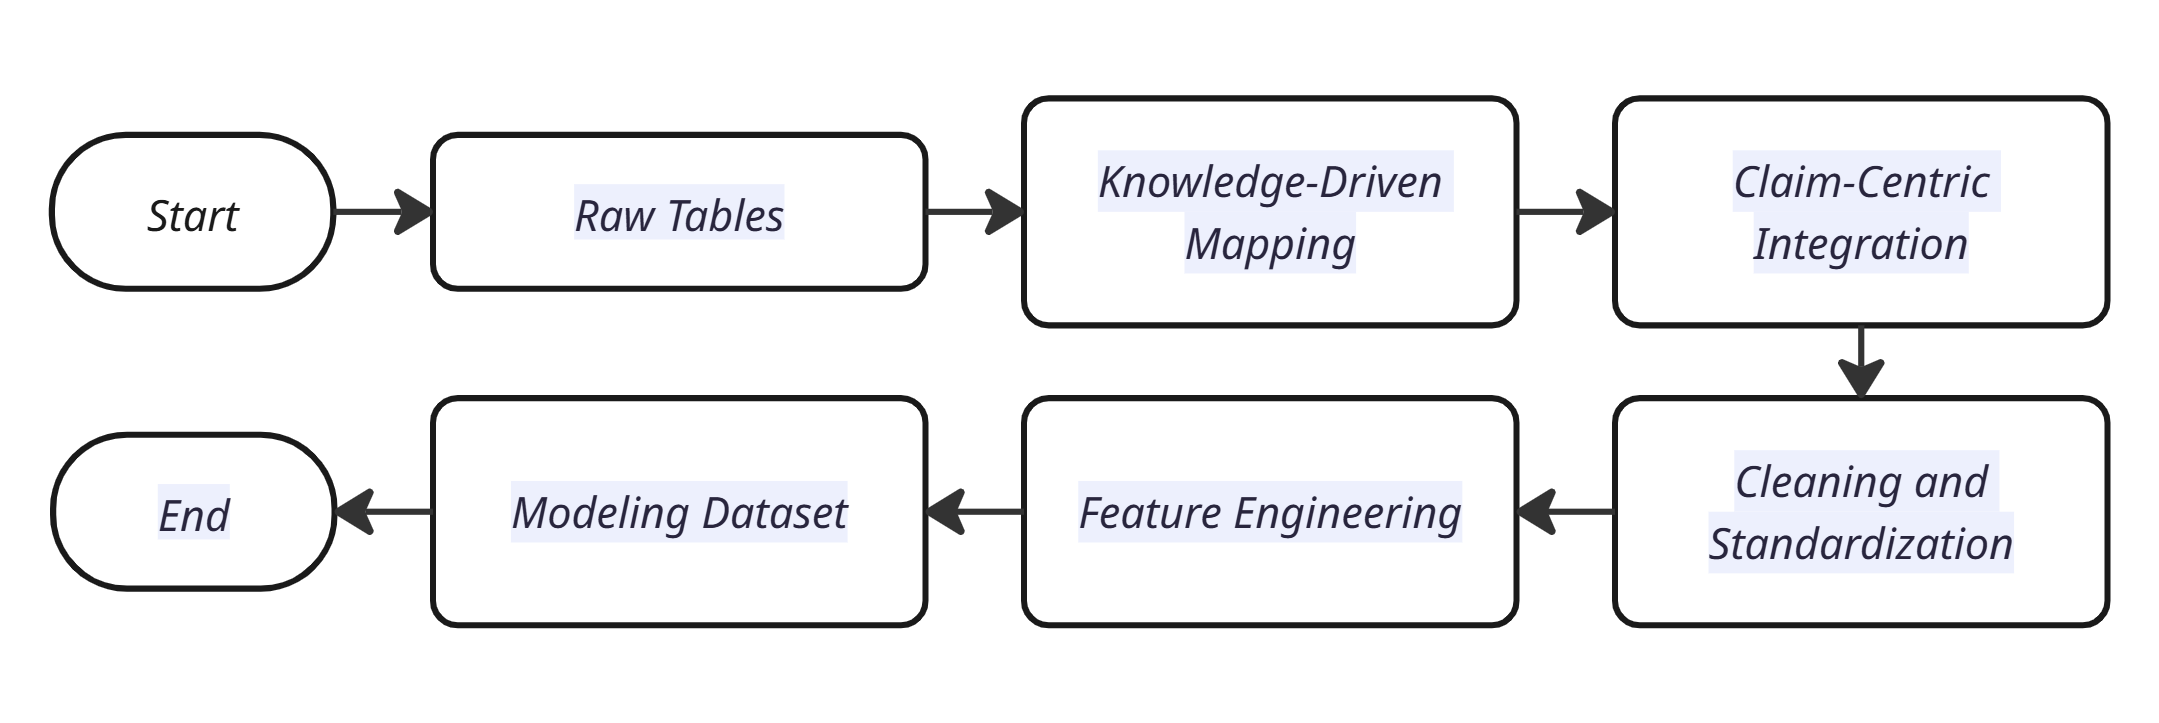
\includegraphics[width=5.51181in,height=1.84583in]{media/media/image7.png}

\phantomsection\label{_Toc228109335}{}Gambar 3. 2 Alur Claim-Centric Data Preparation

Berdasarkan Gambar 3.2, tahap~\emph{Claim-Centric Data Preparation}~dimulai dari pemuatan tabel mentah, dilanjutkan dengan~\emph{knowledge-driven mapping}, integrasi berbasis klaim, pembersihan dan standardisasi data, rekayasa fitur, hingga pembentukan dataset pemodelan. Urutan ini menunjukkan bahwa penyusunan dataset tidak dilakukan secara langsung, melainkan melalui tahapan yang saling bergantung agar data yang dihasilkan bersifat konsisten, informatif, dan siap digunakan pada tahap pemodelan.

Setelah integrasi data selesai, sistem melakukan proses~\emph{cleaning}~dan~\emph{standardization}~untuk memastikan bahwa seluruh variabel berada pada format yang sesuai. Tahap ini mencakup standardisasi identifier, konversi tipe data tanggal, konversi nilai numerik untuk atribut biaya dan tingkat keparahan, serta penanganan nilai kosong dan nilai tidak valid. Proses ini penting karena data yang berasal dari beberapa tabel berbeda berpotensi memiliki format yang tidak seragam. Tanpa standardisasi, kualitas dataset akhir dapat menurun dan memengaruhi performa model pada tahap berikutnya.

Tahap berikutnya adalah~\emph{feature engineering}, yaitu pembentukan variabel turunan yang dirancang untuk menangkap sinyal risiko fraud secara lebih jelas. Fitur yang dibentuk pada penelitian ini dikelompokkan ke dalam beberapa kategori, yaitu fitur demografis, biaya, klinis, diagnosis, histori layanan, dan rasio turunan. Setiap kelompok fitur memiliki tujuan analitis yang berbeda, misalnya untuk menangkap profil peserta, beban biaya klaim, kompleksitas kondisi klinis, maupun pola historis pemanfaatan layanan. Ringkasan kelompok fitur yang digunakan ditunjukkan pada Tabel 3.4.

\phantomsection\label{_Toc228109623}{}Tabel 3. 4 Kelompok Fitur Hasil Rekayasa Fitur

\begin{longtable}[]{@{}
  >{\raggedright\arraybackslash}p{(\columnwidth - 4\tabcolsep) * \real{0.1783}}
  >{\raggedright\arraybackslash}p{(\columnwidth - 4\tabcolsep) * \real{0.5316}}
  >{\raggedright\arraybackslash}p{(\columnwidth - 4\tabcolsep) * \real{0.2901}}@{}}
\toprule\noalign{}
\begin{minipage}[b]{\linewidth}\raggedright
\textbf{Kelompok Fitur}
\end{minipage} & \begin{minipage}[b]{\linewidth}\raggedright
\textbf{Contoh Variabel}
\end{minipage} & \begin{minipage}[b]{\linewidth}\raggedright
\textbf{Tujuan Analitis}
\end{minipage} \\
\midrule\noalign{}
\endhead
\bottomrule\noalign{}
\endlastfoot
Demografis & usia, gender\_singkat & Menggambarkan profil dasar peserta \\
Biaya & tarif\_disetujui, tarif\_inacbg\_dasar, biaya\_per\_hari & Menangkap pola beban biaya klaim \\
Klinis & severity\_level, lama\_rawat\_hari, total\_special\_cmg & Menunjukkan tingkat keparahan dan kompleksitas klinis \\
Diagnosis & jumlah\_diagnosis\_sekunder, jumlah\_grup\_diagnosis\_sekunder & Mengukur intensitas diagnosis tambahan \\
Histori layanan & fktp\_hist\_count\_before, nonkap\_hist\_count\_before & Menangkap pola utilisasi layanan sebelum klaim \\
Rasio turunan & rasio\_tarif\_setuju\_vs\_dasar, rasio\_biaya\_klaim\_vs\_histori\_nonkap & Menyoroti ketidakwajaran relatif antar komponen biaya \\
\end{longtable}

Sebagaimana ditunjukkan pada Tabel 3.4, fitur-fitur hasil rekayasa tidak dibangun secara acak, melainkan disusun berdasarkan hubungan antara informasi administratif, klinis, finansial, dan historis yang terdapat dalam data klaim. Dengan pendekatan ini, dataset akhir tidak hanya memuat variabel mentah, tetapi juga representasi yang lebih kaya untuk menangkap pola potensi fraud atau upcoding.

Keluaran akhir dari tahap ini adalah terbentuknya~model\_df, yaitu dataset pemodelan yang berisi identitas klaim dan variabel-variabel hasil integrasi serta rekayasa fitur yang telah siap dipakai pada tahap pemodelan. Dataset ini menjadi fondasi bagi tahap berikutnya, yaitu~\emph{Hybrid Fraud Detection Modeling}, di mana pseudo-label dibentuk dan model~\emph{supervised learning}~dibandingkan untuk memperoleh konfigurasi deteksi yang paling sesuai.

\subsection{\texorpdfstring{\emph{Hybrid Fraud Detection Modeling}}{Hybrid Fraud Detection Modeling}}\label{hybrid-fraud-detection-modeling}

Tahap~\emph{Hybrid Fraud Detection Modeling}~merupakan inti dari proses analisis pada penelitian ini, karena pada bagian inilah dataset berbasis klaim yang telah dibentuk pada tahap sebelumnya diubah menjadi sistem deteksi risiko yang dapat menghasilkan prediksi. Pendekatan yang digunakan bersifat~\emph{hybrid}, yaitu menggabungkan~\emph{unsupervised learning}~untuk membentuk pseudo-label awal dan~\emph{supervised learning}~untuk membangun model klasifikasi final. Pemilihan pendekatan ini dilakukan untuk menjawab keterbatasan utama pada data klaim, yaitu tidak tersedianya label fraud transaksi riil pada level klaim yang dapat langsung digunakan sebagai target pembelajaran.

Tahap awal dalam komponen ini adalah pemilihan fitur untuk~\emph{unsupervised stage}. Fitur yang digunakan pada tahap ini dipilih dari variabel-variabel numerik yang merepresentasikan karakteristik biaya, klinis, diagnosis, dan histori layanan yang paling relevan untuk mendeteksi anomali pola klaim. Pemilihan fitur pada tahap~\emph{unsupervised}~berbeda dari tahap~\emph{supervised}, karena tujuan utamanya bukan untuk langsung mengklasifikasikan klaim, melainkan untuk membangun dasar penandaan awal terhadap klaim yang memiliki karakteristik menyimpang dari Meioritas populasi.

Pseudo-label kemudian dibentuk menggunakan algoritma~\emph{Isolation Forest}. Algoritma ini digunakan untuk mendeteksi klaim yang memiliki pola anomali berdasarkan kombinasi fitur yang telah dipilih pada tahap sebelumnya. Dalam konteks penelitian ini, klaim yang teridentifikasi sebagai anomali diperlakukan sebagai klaim berisiko dan digunakan sebagai dasar pembentukan pseudo-label. Dengan demikian, sistem dapat menghasilkan target pembelajaran awal tanpa bergantung pada label fraud final yang tidak tersedia secara langsung pada data transaksi klaim.

Setelah proses~\emph{pseudo-labeling}~dilakukan, dataset dibagi menjadi tiga subset utama, yaitu~\emph{train},~\emph{validation}, dan~\emph{test}. Pembagian ini dilakukan untuk menjaga pemisahan fungsi setiap subset, yaitu pelatihan model, pemilihan konfigurasi terbaik, dan evaluasi akhir. Pada tahap ini juga dilakukan~\emph{preprocessing}~agar data siap digunakan oleh model, termasuk penanganan nilai kosong, transformasi variabel numerik, dan pengkodean variabel kategorikal. Alur utama proses pemodelan hybrid dari pseudo-labeling hingga pemilihan model final ditunjukkan pada Gambar 3.3.

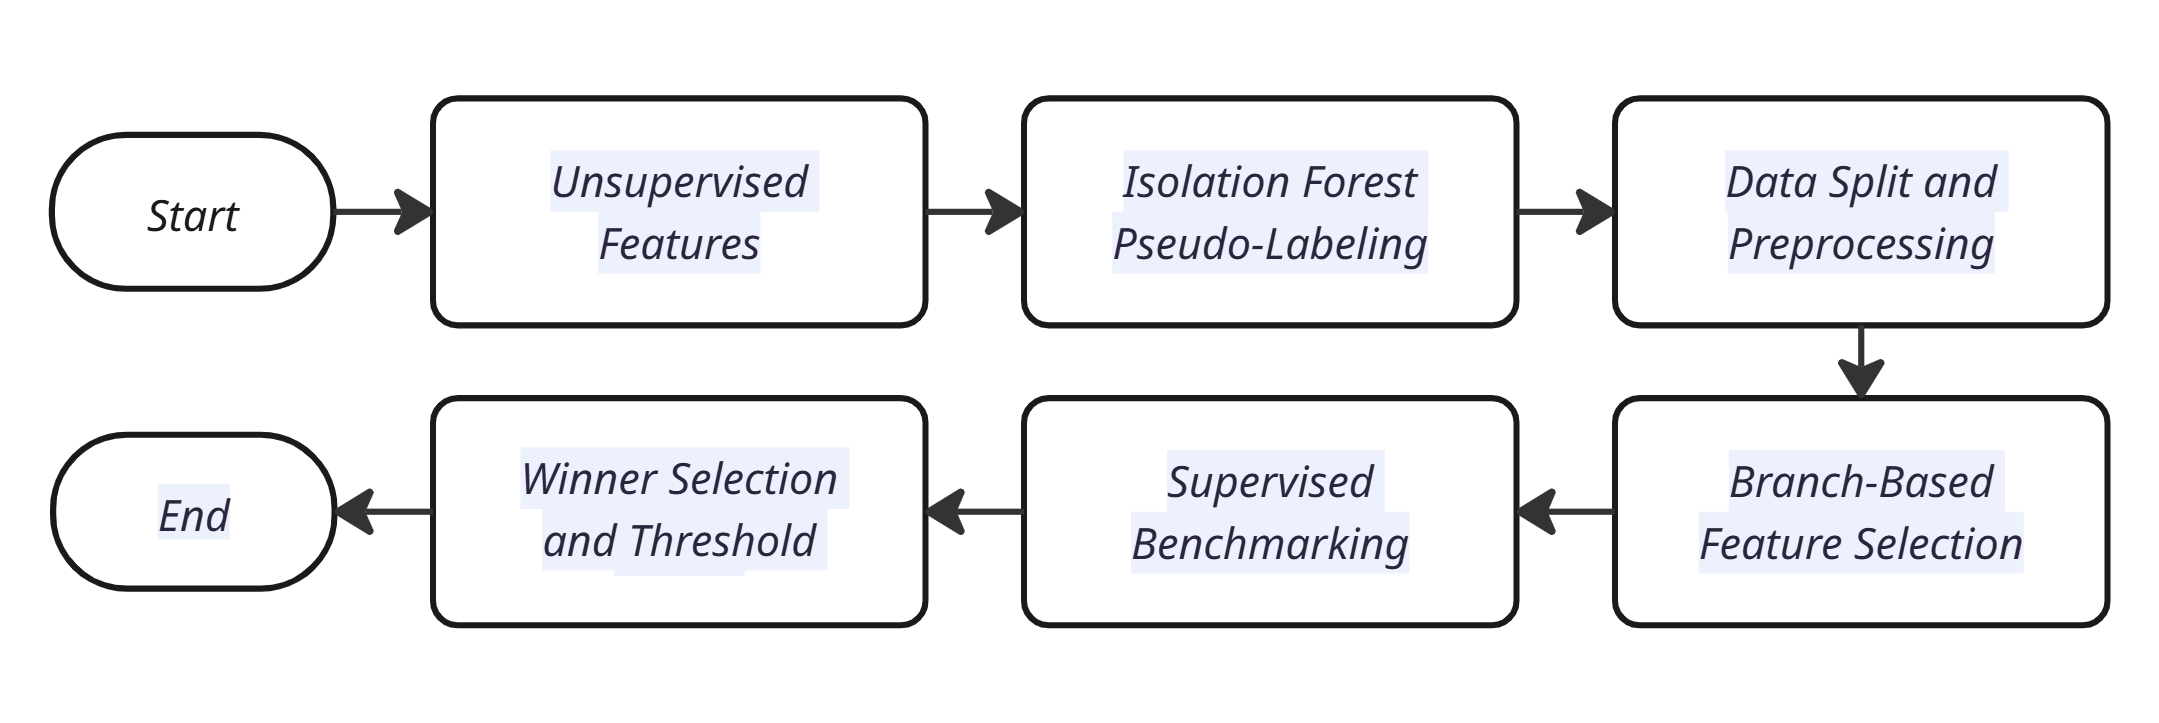
\includegraphics[width=5.51181in,height=1.84583in]{media/media/image8.png}

\phantomsection\label{_Toc228109336}{}Gambar 3. 3 Alur Hybrid Fraud Detection Modeling

Berdasarkan Gambar 3.3, alur pemodelan dimulai dari pemilihan fitur untuk tahap~\emph{unsupervised}, dilanjutkan dengan pembentukan pseudo-label menggunakan~\emph{Isolation Forest}, pembagian data dan~\emph{preprocessing}, seleksi fitur berbasis beberapa cabang,~\emph{benchmarking}~model~\emph{supervised}, hingga pemilihan model terbaik dan penentuan~\emph{threshold}~klasifikasi. Urutan ini menunjukkan bahwa model final pada penelitian ini tidak diperoleh secara langsung dari satu algoritma, melainkan melalui serangkaian tahapan seleksi dan evaluasi yang dirancang untuk menghasilkan konfigurasi deteksi risiko yang paling sesuai.

Setelah~\emph{preprocessing}~dilakukan, sistem menerapkan~\emph{branch-based feature selection}~untuk membandingkan beberapa strategi pemilihan fitur. Pendekatan ini digunakan agar sistem tidak bergantung pada satu skema fitur tunggal, melainkan mengevaluasi beberapa cabang seleksi fitur yang memiliki dasar pertimbangan berbeda. Dengan cara ini, penelitian dapat menilai apakah model memberikan performa terbaik pada fitur yang dipilih secara berbasis pengetahuan domain, berbasis korelasi statistik, berbasis~\emph{variance inflation factor}, berbasis~\emph{permutation importance}, atau pada kombinasi dari beberapa strategi tersebut. Ringkasan branch seleksi fitur yang digunakan ditunjukkan pada Tabel 3.5.

\phantomsection\label{_Toc228109624}{}Tabel 3. 5 Branch Feature Selection yang Digunakan

\begin{longtable}[]{@{}
  >{\raggedright\arraybackslash}p{(\columnwidth - 4\tabcolsep) * \real{0.1862}}
  >{\raggedright\arraybackslash}p{(\columnwidth - 4\tabcolsep) * \real{0.3892}}
  >{\raggedright\arraybackslash}p{(\columnwidth - 4\tabcolsep) * \real{0.4246}}@{}}
\toprule\noalign{}
\begin{minipage}[b]{\linewidth}\raggedright
\textbf{Branch}
\end{minipage} & \begin{minipage}[b]{\linewidth}\raggedright
\textbf{Prinsip Seleksi}
\end{minipage} & \begin{minipage}[b]{\linewidth}\raggedright
\textbf{Tujuan}
\end{minipage} \\
\midrule\noalign{}
\endhead
\bottomrule\noalign{}
\endlastfoot
Domain Expert & Memilih fitur berdasarkan relevansi domain klaim kesehatan & Memastikan fitur penting secara substantif tetap dipertahankan \\
Correlation & Menghapus fitur yang sangat berkorelasi & Mengurangi redundansi antar fitur \\
VIF & Menyeleksi fitur berdasarkan multikolinearitas & Menjaga stabilitas model dan mengurangi ketergantungan antar variabel \\
Permutation & Memilih fitur berdasarkan kontribusi prediktif terhadap model & Mengidentifikasi fitur yang paling berpengaruh terhadap performa \\
Combined & Menggabungkan hasil seleksi dari beberapa strategi & Membentuk himpunan fitur yang lebih seimbang \\
\end{longtable}

Sebagaimana dirangkum pada Tabel 3.5, setiap~\emph{branch}~memiliki prinsip seleksi dan tujuan yang berbeda.~\emph{Branch}~berbasis~\emph{domain expert}~mempertahankan fitur yang dianggap penting secara substantif dalam konteks klaim kesehatan, sedangkan~\emph{branch}~berbasis korelasi dan~\emph{VIF}~berfokus pada pengurangan redundansi antar fitur. Sementara itu,~\emph{branch}~berbasis~\emph{permutation importance}~menekankan kontribusi prediktif fitur terhadap model, dan~\emph{branch combined}~digunakan untuk memperoleh himpunan fitur yang lebih seimbang antara relevansi domain dan stabilitas statistik.

Tahap berikutnya adalah~\emph{supervised benchmarking}, yaitu membandingkan beberapa model klasifikasi untuk mengetahui model mana yang memberikan performa terbaik terhadap pseudo-label yang telah dibentuk. Strategi ini digunakan agar pemilihan model final bersifat empiris dan tidak didasarkan pada asumsi awal terhadap satu algoritma tertentu. Model-model yang dibandingkan pada penelitian ini mencakup model linear, model ensemble berbasis pohon, serta model~\emph{boosting}~yang umum digunakan pada permasalahan klasifikasi tabular. Daftar model yang digunakan dalam proses pembandingan disajikan pada Tabel 3.6.

\phantomsection\label{_Toc228109625}{}Tabel 3. 6 Daftar Model Supervised yang Dibandingkan

\begin{longtable}[]{@{}
  >{\raggedright\arraybackslash}p{(\columnwidth - 4\tabcolsep) * \real{0.1963}}
  >{\raggedright\arraybackslash}p{(\columnwidth - 4\tabcolsep) * \real{0.2972}}
  >{\raggedright\arraybackslash}p{(\columnwidth - 4\tabcolsep) * \real{0.5065}}@{}}
\toprule\noalign{}
\begin{minipage}[b]{\linewidth}\raggedright
\textbf{Model}
\end{minipage} & \begin{minipage}[b]{\linewidth}\raggedright
\textbf{Jenis}
\end{minipage} & \begin{minipage}[b]{\linewidth}\raggedright
\textbf{Fungsi dalam Benchmarking}
\end{minipage} \\
\midrule\noalign{}
\endhead
\bottomrule\noalign{}
\endlastfoot
Logistic Regression & Model linear & Menjadi baseline untuk melihat performa klasifikasi sederhana \\
Random Forest & Ensemble bagging berbasis pohon & Menangkap hubungan nonlinier dan memberikan pembanding model ensemble \\
Linear SVM & Model margin linear & Menjadi pembanding pemisahan kelas pada ruang fitur hasil preprocessing \\
XGBoost & Gradient boosting berbasis pohon & Menguji performa boosting dengan optimasi prediktif tinggi \\
LightGBM & Gradient boosting berbasis histogram & Menjadi pembanding boosting yang efisien pada data tabular \\
CatBoost & Gradient boosting berbasis pohon kategorikal & Menguji kemampuan boosting pada data dengan kombinasi fitur numerik dan kategorikal \\
\end{longtable}

Tabel 3.6 menunjukkan bahwa proses~\emph{benchmarking}~dilakukan secara komparatif terhadap beberapa keluarga model yang memiliki karakteristik berbeda.~\emph{Logistic Regression}~digunakan sebagai model dasar untuk melihat performa pada pola hubungan yang lebih sederhana, sedangkan~\emph{Random Forest},~\emph{XGBoost},~\emph{LightGBM}, dan~\emph{CatBoost}~digunakan untuk menangkap hubungan nonlinier yang lebih kompleks. Selain itu,~\emph{Linear SVM}~digunakan sebagai pembanding tambahan untuk melihat kemampuan pemisahan kelas pada ruang fitur yang telah diproses. Dengan susunan model seperti ini, sistem memiliki dasar evaluasi yang lebih kuat dalam memilih model terbaik.

Hasil dari tahap~\emph{benchmarking}~kemudian digunakan dalam proses~\emph{winner selection}. Pada tahap ini, sistem memilih kombinasi terbaik antara~\emph{branch}~fitur dan model klasifikasi berdasarkan performa evaluasi pada data~\emph{validation}. Setelah model pemenang diperoleh, dilakukan~\emph{threshold tuning}~untuk menentukan ambang klasifikasi yang paling sesuai dengan tujuan deteksi potensi fraud. Proses ini penting karena keputusan akhir model tidak hanya ditentukan oleh probabilitas prediksi, tetapi juga oleh ambang yang digunakan untuk memisahkan klaim berisiko dan klaim normal.

Untuk memudahkan pemahaman hubungan antar tahap pada komponen ini, ringkasan alur pemodelan hybrid dapat disajikan pada Tabel 3.7. Tabel tersebut merangkum input, proses, dan output pada setiap tahap utama, sehingga pembaca dapat melihat keterkaitan antara pembentukan pseudo-label, seleksi fitur, pembandingan model, hingga pemilihan model final secara lebih cepat dan sistematis.

\phantomsection\label{_Toc228109626}{}Tabel 3. 7 Ringkasan Tahap Pemodelan Hybrid

\begin{longtable}[]{@{}
  >{\raggedright\arraybackslash}p{(\columnwidth - 6\tabcolsep) * \real{0.2368}}
  >{\raggedright\arraybackslash}p{(\columnwidth - 6\tabcolsep) * \real{0.2240}}
  >{\raggedright\arraybackslash}p{(\columnwidth - 6\tabcolsep) * \real{0.3020}}
  >{\raggedright\arraybackslash}p{(\columnwidth - 6\tabcolsep) * \real{0.2372}}@{}}
\toprule\noalign{}
\begin{minipage}[b]{\linewidth}\raggedright
\textbf{Tahap}
\end{minipage} & \begin{minipage}[b]{\linewidth}\raggedright
\textbf{Input}
\end{minipage} & \begin{minipage}[b]{\linewidth}\raggedright
\textbf{Proses}
\end{minipage} & \begin{minipage}[b]{\linewidth}\raggedright
\textbf{Output}
\end{minipage} \\
\midrule\noalign{}
\endhead
\bottomrule\noalign{}
\endlastfoot
Pemilihan fitur unsupervised & Dataset hasil data preparation & Menentukan fitur numerik yang relevan untuk deteksi anomali & Set fitur unsupervised \\
Pseudo-labeling & Fitur unsupervised & Mendeteksi anomali menggunakan Isolation Forest & Anomaly score dan pseudo-label \\
Data split dan preprocessing & Dataset dengan pseudo-label & Membagi data dan menyiapkan fitur numerik serta kategorikal & Train, validation, test yang siap model \\
Branch-based feature selection & Data train hasil preprocessing & Menyeleksi fitur melalui beberapa branch & Beberapa kandidat set fitur \\
Supervised benchmarking & Data train dan validation & Membandingkan performa beberapa model klasifikasi & Hasil benchmarking model \\
Winner selection dan threshold tuning & Hasil benchmarking & Memilih model terbaik dan menentukan threshold klasifikasi & Model final dan threshold terbaik \\
\end{longtable}

Berdasarkan Tabel 3.7, dapat dilihat bahwa komponen~\emph{Hybrid Fraud Detection Modeling}~tidak hanya berfungsi sebagai tahap pelatihan model, tetapi juga sebagai kerangka seleksi bertingkat yang memastikan model final diperoleh melalui proses yang terkontrol. Tahap ini menghasilkan model terbaik beserta konfigurasi ambang klasifikasi yang selanjutnya digunakan pada komponen evaluasi dan interpretabilitas hasil.

\subsection{\texorpdfstring{\emph{Evaluation and Interpretability}}{Evaluation and Interpretability}}\label{evaluation-and-interpretability}

Tahap~\emph{Evaluation and Interpretability}~merupakan komponen akhir dalam perancangan sistem yang bertujuan menilai performa model final sekaligus menjelaskan alasan di balik prediksi yang dihasilkan. Pada penelitian ini, evaluasi tidak hanya diarahkan untuk mengetahui seberapa baik model membedakan klaim berisiko dan klaim normal, tetapi juga untuk memastikan bahwa hasil prediksi dapat ditafsirkan secara analitis. Pendekatan ini penting karena sistem deteksi fraud pada data klaim kesehatan harus mampu memberikan dasar penjelasan yang kuat, sehingga hasil yang diperoleh tidak berhenti pada skor risiko semata, melainkan dapat digunakan sebagai bahan pendukung untuk proses pemeriksaan lebih lanjut.

Setelah model pemenang dan~\emph{threshold}~klasifikasi diperoleh pada tahap sebelumnya, sistem melakukan~\emph{final model evaluation}~pada data~\emph{test}~yang tidak terlibat dalam proses pemilihan model. Evaluasi ini digunakan untuk menggambarkan kemampuan generalisasi model terhadap data yang belum pernah dilihat sebelumnya. Dengan demikian, performa yang diperoleh pada tahap ini merepresentasikan kualitas model final secara lebih objektif dibandingkan hasil evaluasi pada data pelatihan atau validasi.

Evaluasi model pada penelitian ini menggunakan beberapa metrik utama, yaitu~\emph{F1-score},~\emph{PR-AUC},~\emph{ROC-AUC},~\emph{precision},~\emph{recall}, dan~\emph{Matthews Correlation Coefficient}~(MCC). Pemilihan metrik tersebut didasarkan pada karakteristik permasalahan deteksi fraud, di mana distribusi kelas tidak seimbang dan kesalahan prediksi memiliki implikasi yang berbeda. Ringkasan metrik yang digunakan beserta fungsi dan alasan penggunaannya disajikan pada Tabel 3.8.

\phantomsection\label{_Toc228109627}{}Tabel 3. 8 Metrik Evaluasi Model

\begin{longtable}[]{@{}
  >{\raggedright\arraybackslash}p{(\columnwidth - 4\tabcolsep) * \real{0.1443}}
  >{\raggedright\arraybackslash}p{(\columnwidth - 4\tabcolsep) * \real{0.3429}}
  >{\raggedright\arraybackslash}p{(\columnwidth - 4\tabcolsep) * \real{0.5128}}@{}}
\toprule\noalign{}
\begin{minipage}[b]{\linewidth}\raggedright
\textbf{Metrik}
\end{minipage} & \begin{minipage}[b]{\linewidth}\raggedright
\textbf{Fungsi}
\end{minipage} & \begin{minipage}[b]{\linewidth}\raggedright
\textbf{Alasan Digunakan}
\end{minipage} \\
\midrule\noalign{}
\endhead
\bottomrule\noalign{}
\endlastfoot
F1-score & Mengukur keseimbangan antara precision dan recall & Cocok untuk deteksi fraud yang menuntut keseimbangan antara penangkapan kasus berisiko dan pengendalian kesalahan prediksi \\
PR-AUC & Mengukur kualitas pemeringkatan prediksi pada kelas positif & Relevan untuk data yang tidak seimbang karena lebih fokus pada kemampuan model mengenali klaim berisiko \\
ROC-AUC & Mengukur kemampuan model membedakan dua kelas secara umum & Memberikan gambaran umum separabilitas model \\
Precision & Mengukur proporsi klaim yang diprediksi berisiko dan benar-benar berisiko & Penting untuk menghindari terlalu banyak klaim normal yang salah ditandai \\
Recall & Mengukur proporsi klaim berisiko yang berhasil ditangkap model & Penting agar klaim berisiko tidak banyak terlewat \\
MCC & Mengukur kualitas klasifikasi secara seimbang & Cocok untuk kondisi kelas tidak seimbang karena mempertimbangkan seluruh komponen confusion matrix \\
\end{longtable}

Sebagaimana ditunjukkan pada Tabel 3.8, metrik evaluasi yang digunakan tidak hanya berfokus pada satu aspek performa.~\emph{Precision}~diperlukan untuk melihat ketepatan model dalam menandai klaim berisiko, sedangkan~\emph{recall}~diperlukan untuk menilai kemampuan model dalam menangkap klaim yang seharusnya tidak terlewat.~\emph{F1-score}~digunakan sebagai ukuran keseimbangan antara keduanya. Selain itu,~\emph{PR-AUC}~dan~\emph{ROC-AUC}~digunakan untuk menilai kualitas pemeringkatan skor prediksi, sedangkan~\emph{MCC}~digunakan karena mampu memberikan gambaran performa klasifikasi yang lebih seimbang pada kondisi distribusi kelas yang tidak merata.

Selain evaluasi performa, sistem ini juga dirancang untuk memberikan interpretasi terhadap hasil prediksi model. Interpretabilitas dilakukan pada dua tingkatan, yaitu interpretasi global dan interpretasi lokal. Interpretasi global digunakan untuk memahami fitur-fitur yang secara umum paling berpengaruh terhadap keputusan model, sedangkan interpretasi lokal digunakan untuk menjelaskan prediksi pada klaim tertentu yang memiliki tingkat risiko tinggi. Alur umum tahap evaluasi dan interpretabilitas pada penelitian ini ditunjukkan pada Gambar 3.4.

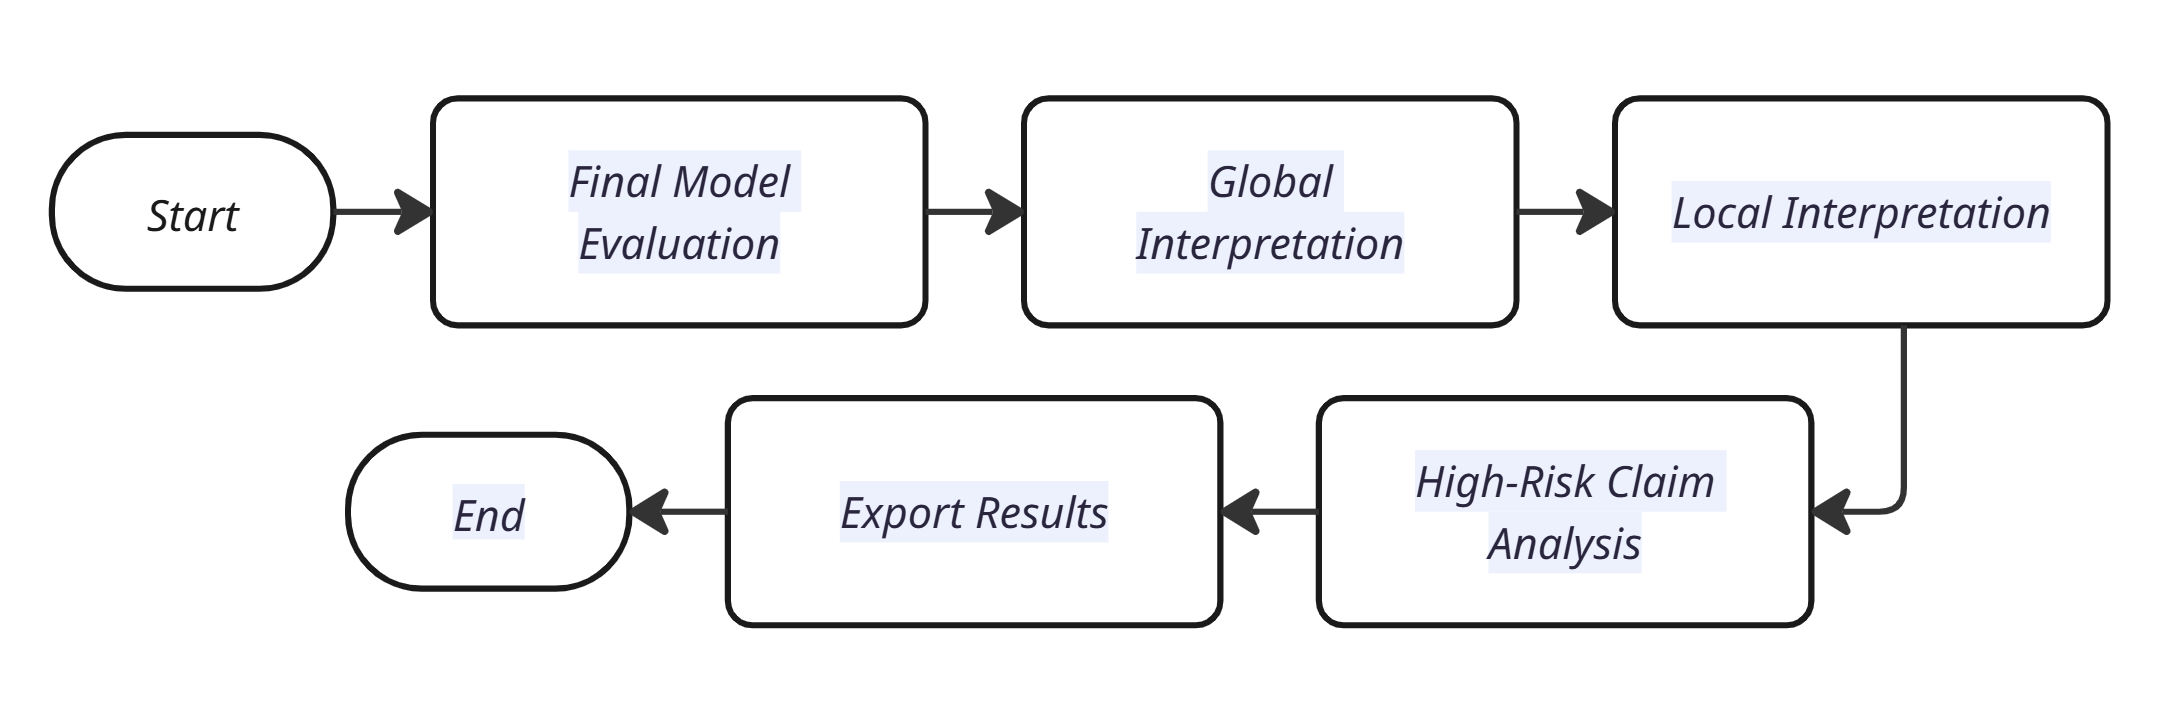
\includegraphics[width=5.51181in,height=1.84583in]{media/media/image9.png}

\phantomsection\label{_Toc228109337}{}Gambar 3. 4 Alur Evaluation and Interpretability

Berdasarkan Gambar 3.4, tahap ini dimulai dari evaluasi model final, kemudian dilanjutkan dengan interpretasi global, interpretasi lokal, analisis klaim berisiko tinggi, dan ekspor artefak hasil. Susunan ini menunjukkan bahwa keluaran sistem tidak hanya berupa angka performa, tetapi juga mencakup penjelasan fitur-fitur yang memengaruhi prediksi dan daftar klaim yang layak diprioritaskan untuk analisis lanjutan.

Interpretasi global pada penelitian ini dilakukan melalui~\emph{feature importance}~dan~\emph{SHAP}.~\emph{Feature importance}~digunakan untuk memberikan gambaran umum mengenai variabel mana yang paling dominan dalam proses pengambilan keputusan model. Sementara itu,~\emph{SHAP}~digunakan untuk menjelaskan arah dan besar kontribusi setiap fitur terhadap prediksi model secara lebih rinci. Dengan memadukan kedua teknik ini, penelitian tidak hanya memperoleh daftar fitur yang penting, tetapi juga dapat memahami bagaimana perubahan nilai suatu fitur berasosiasi dengan peningkatan atau penurunan risiko klaim.

Selain interpretasi global, penelitian ini juga menggunakan~\emph{Partial Dependence Plot}~(PDP) untuk melihat pola hubungan antara perubahan nilai fitur tertentu terhadap probabilitas fraud yang diprediksi model. Teknik ini membantu memperjelas bagaimana suatu fitur memengaruhi keluaran model secara rata-rata pada populasi data. Dengan demikian, PDP menjadi pelengkap interpretasi global karena tidak hanya menunjukkan pentingnya fitur, tetapi juga menggambarkan kecenderungan pengaruh fitur tersebut terhadap keputusan model.

Pada tingkat interpretasi lokal, penelitian ini menggunakan~\emph{LIME}~untuk menjelaskan prediksi pada klaim tertentu secara individual. Teknik ini digunakan untuk melihat fitur-fitur yang mendorong model memberikan skor risiko tinggi pada klaim tertentu. Dengan pendekatan ini, analisis tidak berhenti pada level populasi, tetapi juga masuk ke level observasi individual yang relevan untuk proses investigasi. Ringkasan teknik interpretabilitas yang digunakan pada penelitian ini disajikan pada Tabel 3.9.

\phantomsection\label{_Toc228109628}{}Tabel 3. 9 Teknik Interpretabilitas yang Digunakan

\begin{longtable}[]{@{}
  >{\raggedright\arraybackslash}p{(\columnwidth - 4\tabcolsep) * \real{0.2124}}
  >{\raggedright\arraybackslash}p{(\columnwidth - 4\tabcolsep) * \real{0.2017}}
  >{\raggedright\arraybackslash}p{(\columnwidth - 4\tabcolsep) * \real{0.5858}}@{}}
\toprule\noalign{}
\begin{minipage}[b]{\linewidth}\raggedright
\textbf{Teknik}
\end{minipage} & \begin{minipage}[b]{\linewidth}\raggedright
\textbf{Jenis}
\end{minipage} & \begin{minipage}[b]{\linewidth}\raggedright
\textbf{Tujuan}
\end{minipage} \\
\midrule\noalign{}
\endhead
\bottomrule\noalign{}
\endlastfoot
\emph{Feature Importance} & Interpretasi global & Mengidentifikasi fitur yang paling dominan dalam keputusan model secara umum \\
SHAP & Interpretasi global & Menjelaskan arah dan besar kontribusi fitur terhadap prediksi model \\
PDP & Interpretasi global & Menggambarkan pola pengaruh perubahan nilai fitur terhadap probabilitas prediksi \\
LIME & Interpretasi lokal & Menjelaskan alasan prediksi model pada klaim individual \\
\end{longtable}

Sebagaimana dirangkum pada Tabel 3.9, setiap teknik interpretabilitas memiliki fungsi yang berbeda dan saling melengkapi.~\emph{Feature importance}~memberikan gambaran prioritas fitur pada level global,~\emph{SHAP}~memperkaya interpretasi global dengan kontribusi fitur yang lebih rinci,~\emph{PDP}~menjelaskan pola pengaruh fitur terhadap probabilitas prediksi, dan~\emph{LIME}~digunakan untuk membaca alasan prediksi pada klaim individual. Kombinasi teknik-teknik tersebut membuat hasil model lebih mudah dipahami dan lebih relevan untuk digunakan dalam analisis risiko klaim.

Tahap berikutnya adalah analisis klaim berisiko tinggi. Pada bagian ini, sistem menyusun daftar klaim dengan probabilitas fraud tertinggi berdasarkan hasil prediksi model final. Klaim-klaim tersebut kemudian menjadi objek analisis lokal untuk melihat faktor apa saja yang paling berkontribusi terhadap penilaian risiko. Dengan cara ini, sistem tidak hanya menghasilkan klasifikasi, tetapi juga mendukung proses prioritisasi klaim yang memerlukan telaah lebih lanjut.

Seluruh keluaran penting dari tahap evaluasi dan interpretabilitas selanjutnya disimpan dalam bentuk artefak hasil. Artefak ini mencakup informasi model pemenang, analisis~\emph{threshold}, daftar klaim berisiko tinggi, metrik evaluasi akhir, serta laporan interpretabilitas. Penyimpanan artefak dilakukan agar hasil penelitian dapat digunakan kembali pada proses pelaporan, dokumentasi, maupun analisis lanjutan. Ringkasan artefak yang diekspor pada penelitian ini disajikan pada Tabel 3.10.

\phantomsection\label{_Toc228109629}{}Tabel 3. 10 Artefak Hasil yang Diekspor

\begin{longtable}[]{@{}
  >{\raggedright\arraybackslash}p{(\columnwidth - 4\tabcolsep) * \real{0.2389}}
  >{\raggedright\arraybackslash}p{(\columnwidth - 4\tabcolsep) * \real{0.3520}}
  >{\raggedright\arraybackslash}p{(\columnwidth - 4\tabcolsep) * \real{0.4091}}@{}}
\toprule\noalign{}
\begin{minipage}[b]{\linewidth}\raggedright
\textbf{Nama Artefak}
\end{minipage} & \begin{minipage}[b]{\linewidth}\raggedright
\textbf{Isi}
\end{minipage} & \begin{minipage}[b]{\linewidth}\raggedright
\textbf{Kegunaan}
\end{minipage} \\
\midrule\noalign{}
\endhead
\bottomrule\noalign{}
\endlastfoot
\emph{winner info} & Informasi model pemenang, \emph{branch} terbaik, dan \emph{threshold final} & Mendokumentasikan konfigurasi final sistem \\
\emph{threshold analysis} & Ringkasan evaluasi \emph{threshold} klasifikasi & Menentukan ambang keputusan model yang paling sesuai \\
\emph{top-risk claims} & Daftar klaim dengan probabilitas \emph{fraud} tertinggi & Mendukung prioritisasi klaim untuk analisis lanjutan \\
\emph{final metrics} & Ringkasan metrik evaluasi model final & Mendukung pembahasan performa sistem \\
laporan \emph{interpretability} & Hasil \emph{feature importance}, SHAP, PDP, dan LIME & Menjelaskan alasan di balik prediksi model \\
\end{longtable}

Berdasarkan Tabel 3.10, artefak hasil memiliki fungsi yang berbeda-beda tetapi saling mendukung. Informasi model pemenang dan~\emph{threshold analysis}~digunakan untuk mendokumentasikan konfigurasi final sistem, sedangkan~\emph{top-risk claims}~dan~\emph{final metrics}~digunakan untuk mendukung pembahasan hasil eksperimen. Sementara itu, laporan interpretabilitas digunakan untuk menjelaskan hubungan antara prediksi model dan karakteristik klaim yang dianalisis. Dengan adanya artefak ini, keluaran penelitian menjadi lebih terstruktur dan siap digunakan sebagai dasar penulisan hasil pada bab berikutnya.

\emph{(Halaman ini sengaja dikosongkan)}
